\documentclass{article}

% if you need to pass options to natbib, use, e.g.:
% \PassOptionsToPackage{numbers, compress}{natbib}
% before loading nips_2016
%
% to avoid loading the natbib package, add option nonatbib:
% \usepackage[nonatbib]{nips_2016}

%\usepackage{nips_2016}

% to compile a camera-ready version, add the [final] option, e.g.:
\usepackage[final]{nips_2016}

\usepackage[utf8]{inputenc} % allow utf-8 input
\usepackage[T1]{fontenc}    % use 8-bit T1 fonts
\usepackage{hyperref}       % hyperlinks
\usepackage{url}            % simple URL typesetting
\usepackage{booktabs}       % professional-quality tables
\usepackage{amsfonts}       % blackboard math symbols
\usepackage{nicefrac}       % compact symbols for 1/2, etc.
\usepackage{microtype}      % microtypography
\usepackage{color}
\usepackage{graphicx}
\graphicspath{ {../figures/} }
\usepackage{subcaption}

\title{Formatting instructions for NIPS 2016}

% The \author macro works with any number of authors. There are two
% commands used to separate the names and addresses of multiple
% authors: \And and \AND.
%
% Using \And between authors leaves it to LaTeX to determine where to
% break the lines. Using \AND forces a line break at that point. So,
% if LaTeX puts 3 of 4 authors names on the first line, and the last
% on the second line, try using \AND instead of \And before the third
% author name.

\author{
  Elijahu Ben-Michael \\
  Department of Statistics\\
  UC Berkeley
  %% examples of more authors
   \And
  Runjing Liu \\
  Department of Statistics\\
  UC Berkeley
  %% \texttt{email} \\
   \AND
  Jake Soloff \\
  Department of Statistics\\
  UC Berkeley
  %% \texttt{email} \\
  %% \And
  %% Coauthor \\
  %% Affiliation \\
  %% Address \\
  %% \texttt{email} \\
  %% \And
  %% Coauthor \\
  %% Affiliation \\
  %% Address \\
  %% \texttt{email} \\
}

\begin{document}
% \nipsfinalcopy is no longer used

\maketitle

\begin{abstract}
  The abstract paragraph should be indented \nicefrac{1}{2}~inch
  (3~picas) on both the left- and right-hand margins. Use 10~point
  type, with a vertical spacing (leading) of 11~points.  The word
  \textbf{Abstract} must be centered, bold, and in point size 12. Two
  line spaces precede the abstract. The abstract must be limited to
  one paragraph.
\end{abstract}

\section{Introduction}
Quantitative analysis of legislative data has the potential to provide new insights into how our government functions. 





\subsection{Motivation} 
Voting records of legislators are commonly used by political scientists to examine relationships between legislator policy preferences, institutional structures, and legislative outcomes (Clinton et al 2004). In fact, even simple dimensionality reduction techniques on roll call data are able to uncover the political charactristics of individual representatives such as party affiliation. In figure \ref{fig:NNMF}, we factored the $448\times1707$ matrix representing the 448 representatives and the 1707 bills they voted on into two nonnegative matrices of sizes $448\times 2$ and $2\times 1707$ . Plotting the  $448\times 2$ matrix where each row places a representative in a two dimensional space, we see that party affiliation is clearly clustered. \par

Another dimensionality technque we applied to visualize voting data was principle component analysis (figure \ref{fig:PCA}). We formed the principle components by computing the two largest eigenvalues and their respective eigenvectors on the $448\times 448$ covariance matrix of vote data, and the representative's voting profiles were projected onto the space onto these components. Again, we see that party affiliatoin is clearly clustered. 



\begin{figure}[h]
  \centering
    \begin{subfigure}[b]{0.4\textwidth}
        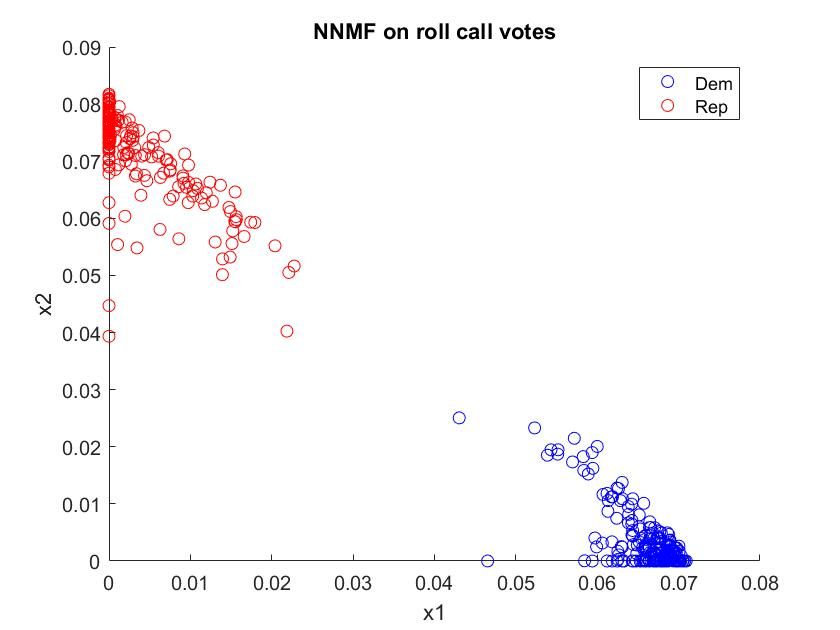
\includegraphics[width=\textwidth]{NNMF_votes.jpg}
        \caption{}
        \label{fig:NNMF}
    \end{subfigure}
          \begin{subfigure}[b]{0.4\textwidth}
        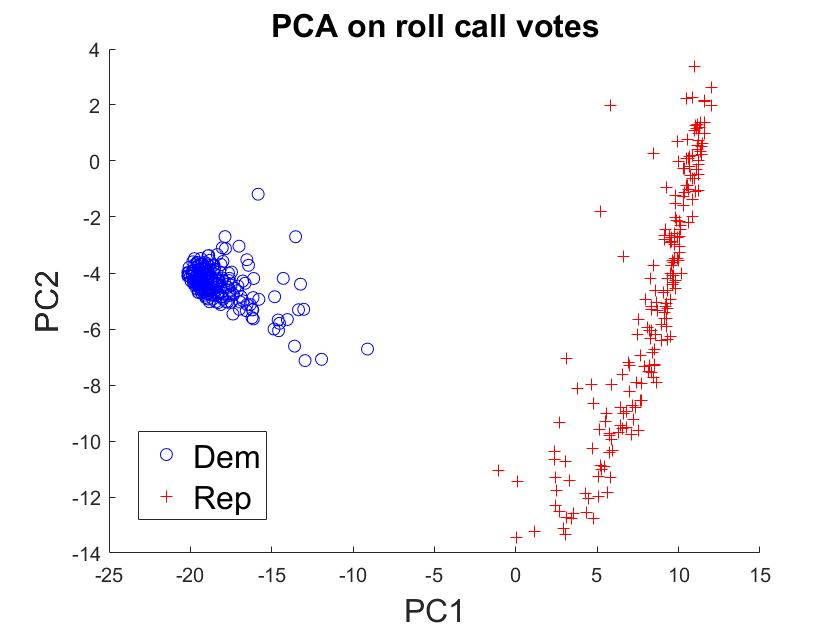
\includegraphics[width=\textwidth]{PCA_votes}
        \caption{}
        \label{fig:PCA}
    \end{subfigure}
  \caption{(a) Nonnegative matrix factoriation on the $448\times 1707$ matrix (448 representatives, 1707 bills) of roll call votes; (b) Principle component analysis on the covariance matrix of roll call vote data}
\end{figure}

Another common analysis of roll call vote data is to conduct {\itshape ideal point modeling}. {\color{red} maybe the next sentences goes in the introduction \{} Here, a congressman and a bill is presumed to lie in a latent `'ideoloigcal space,'' where the probability of a ``yay'' or ``nay'' response is a function of the bill's position and the congressman's position. The congressman's position is known as an `'ideal point'' because his or her utility decreases as a bill's position deviates from this point. {\color{red} \}}

In Gerrish and Blei 2011, ideal points of each senator were drawn from a zero mean Gaussian prior. To obtain better estimates of the representatives' ideal points, we incorporate data from caucus memberships because we hypothesize that sharing caucuses with other representatives can sway a representative's voting behavior. Figure \ref{fig:Nhood_Caucus} shows the relationship between representatives within several caucuses. We first used roll call vote data to infer an undirected graphical model on the entire House in which each node denotes a representative. We assumed a pairwise interactions describe via an Ising model in which a binary variable of a representative voting either yes or no was placed on each node. The edges were inferred using neighborhood selection. We found that the connectivity (\#edges /\#nodes(\#nodes-1) ) of the full graph of 448 representatives to be 0.064, while the connectivity within subgraphs corresponding to a caucuses was much higher. This sugggests that a representative more likely to be influenced by a member of his caucus than a random other representative in the House. Therefore, we hope that using caucus data to infer community membership will enable us to better predict roll call votes. By incorporating more data to estimate ideal points, we hope to be able to extend the one dimensional ideological space in Gerrish and Blei to higher dimensions. In doing so, we hypothesize that more accurate predictions of roll call votes can be explained. 


% The connection between caucus memberships and ideal points are described by a {\itshape stochastic block model} (see below). 

%This model posits that the representatives are grouped by latent communites, and these communities manifest themselves in a representative's ideal point (representatives in the same community are likely to have similar ideal points) and in a representative's caucus membership (representatives in the same community are likely to share many caucuses). 




\begin{figure}[h]
  \centering
    \begin{subfigure}[b]{0.49\textwidth}
        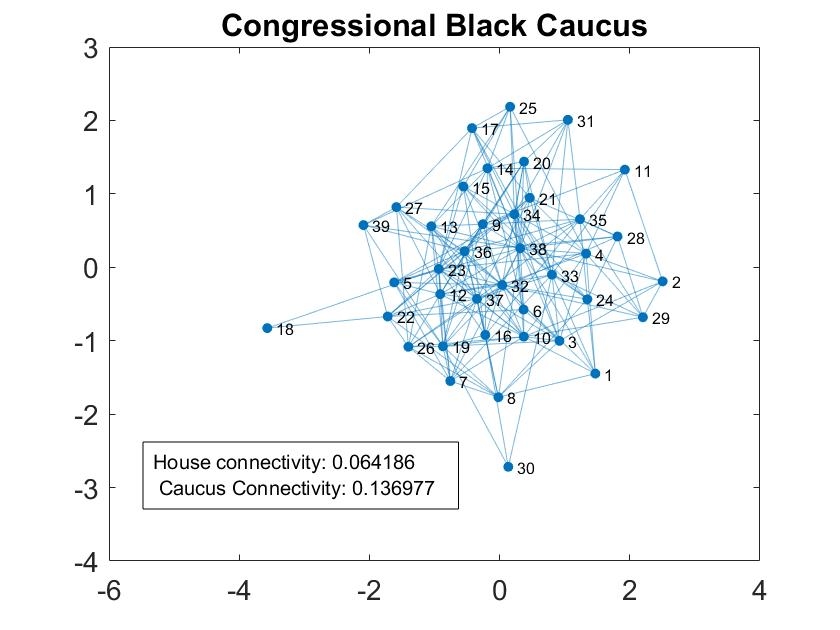
\includegraphics[width=\textwidth]{/Neighborhood_Regression/Congressional_Black_Caucus.jpg}
        \caption{}
    \end{subfigure}
          \begin{subfigure}[b]{0.49\textwidth}
        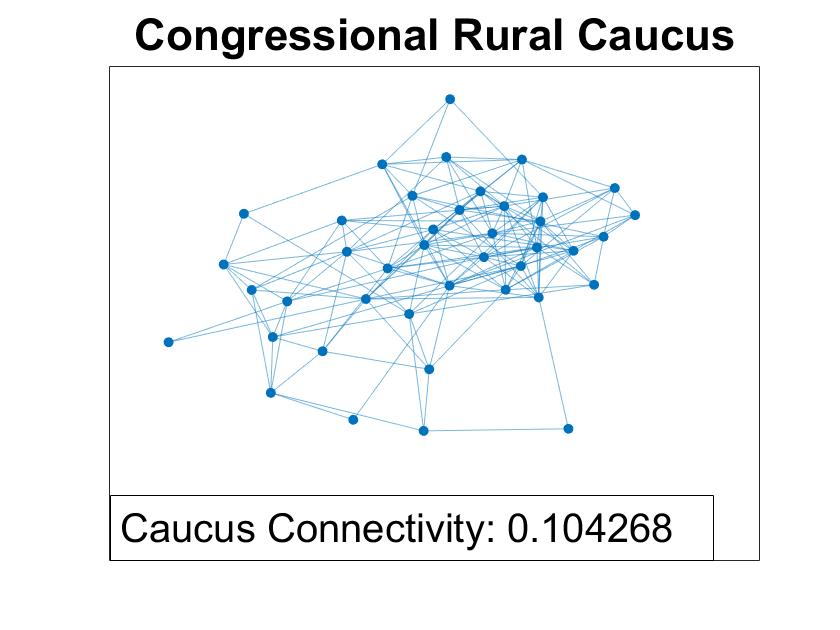
\includegraphics[width=\textwidth]{/Neighborhood_Regression/Congr_Rural_Caucus.jpg}
        \caption{}
    \end{subfigure}
        \begin{subfigure}[b]{0.49\textwidth}
        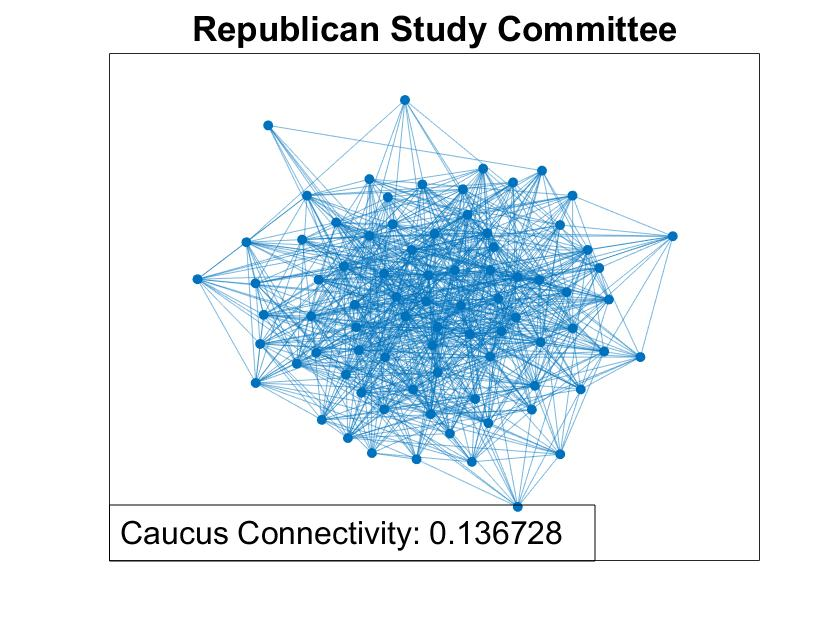
\includegraphics[width=\textwidth]{/Neighborhood_Regression/Rep_Study_Committee.jpg}
        \caption{}
    \end{subfigure}
          \begin{subfigure}[b]{0.49\textwidth}
        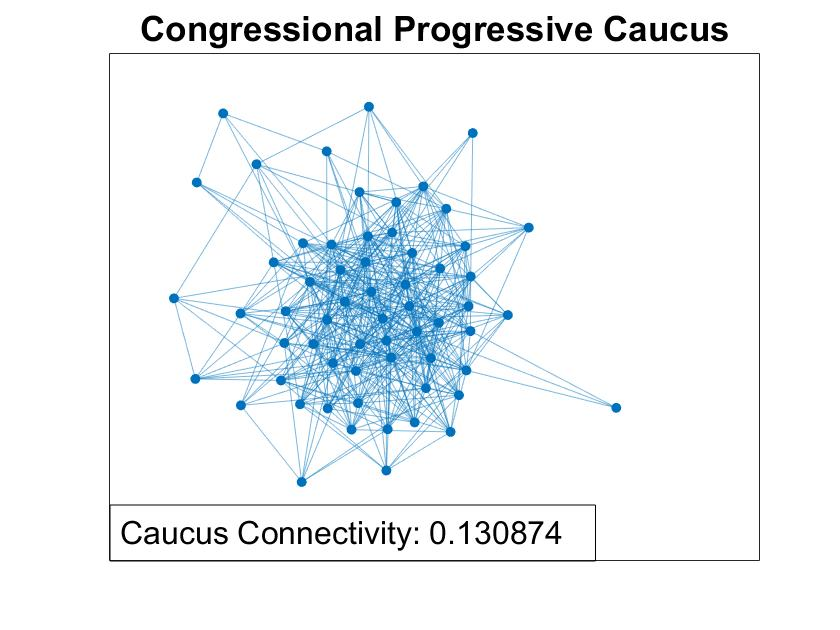
\includegraphics[width=\textwidth]{/Neighborhood_Regression/Congr_Prog_Caucus.jpg}
        \caption{}
    \end{subfigure}
  \caption{Graphs inferred from Neighborhood regression on House roll call vote data. Shown here are subgraphs with senators taken from a given caucus. The caucuses are their connetivities shown here are (a) the Congressional Black Caucus, connectivity 0.137; (b) the Congressional Rural Caucus, connectivity 0.104; (c) the Republican Study Committee, connectivity 0.136; and (d) the Congressional Progressive Caucus, connectivity 0.131. In each case, the connectivity within the caucuses was higher than the connectivity of the whole graph of the House (0.064). {\color{red} note to bliu make figure font bigger} }
      \label{fig:Nhood_Caucus}
\end{figure}




\section{The model}
\subsection{Ideal point model}




\subsection{Stochastic Block Model}


\section{Results}

\section{Discussion}




\section*{References}

\medskip

\small

[1] Gerrish, S.M.\ \& Blei, M.B. \ (2011) Predicting Legislative Roll Calls from Text. {\it Proceedings of the 28th International Conference on Machine Learning}

\appendix

\section{Variational updates}

\end{document}